%
% Modified by Megan Patnott
% Last Change: Jan 18, 2013
%
%%%%%%%%%%%%%%%%%%%%%%%%%%%%%%%%%%%%%%%%%%%%%%%%%%%%%%%%%%%%%%%%%%%%%%%%
%
% Modified by Sameer Vijay
% Last Change: Tue Jul 26 2005 13:00 CEST
%
%%%%%%%%%%%%%%%%%%%%%%%%%%%%%%%%%%%%%%%%%%%%%%%%%%%%%%%%%%%%%%%%%%%%%%%%
%
% Sample Notre Dame Thesis/Dissertation
% Using Donald Peterson's ndthesis classfile
%
% Written by Jeff Squyres and Don Peterson
%
% Provided by the Information Technology Committee of
%   the Graduate Student Union
%   http://www.gsu.nd.edu/
%
% Nothing in this document is serious except the format.  :-)
%
% If you have any suggestions, comments, questions, please send e-mail
% to: ndthesis@gsu.nd.edu
%
%%%%%%%%%%%%%%%%%%%%%%%%%%%%%%%%%%%%%%%%%%%%%%%%%%%%%%%%%%%%%%%%%%%%%%%%


%
% Chapter 6
%

\chapter{Discussion}

\section{Dynamic Moments of Inertia}
\label{sec:Dynamic}

Something something moment of inertia.

\subsection{Bands in $^{154}$Gd}
\label{sec:154_Dynamic}

To examine the structure of the bands seen in this experiment, the dynamic moments of inertia can be compared. This is usually done with higher spins, but examination at lower spins can allow for more bands to be compared. The energy difference tracks linearly, with the slope being directly correlated to the moment of inertia of the band, as seen in Figure \ref{fig:154_Dynamic0} and Figure \ref{fig:154_Dynamic}. The slopes of these bands are summarized in Table \ref{tab:154_Dynamic}. Slopes with an error had enough points to calculate the error on the slope. Those without error had only two points or, in the case of the second excited $2^+$ band, one point and the origin. These points each require two levels of the band to be known for calculation. The intercept was left to float, but not included, as it was in agreement with 0 in all cases where error could be calculated.

\begin{figure}[!]
    \centering
    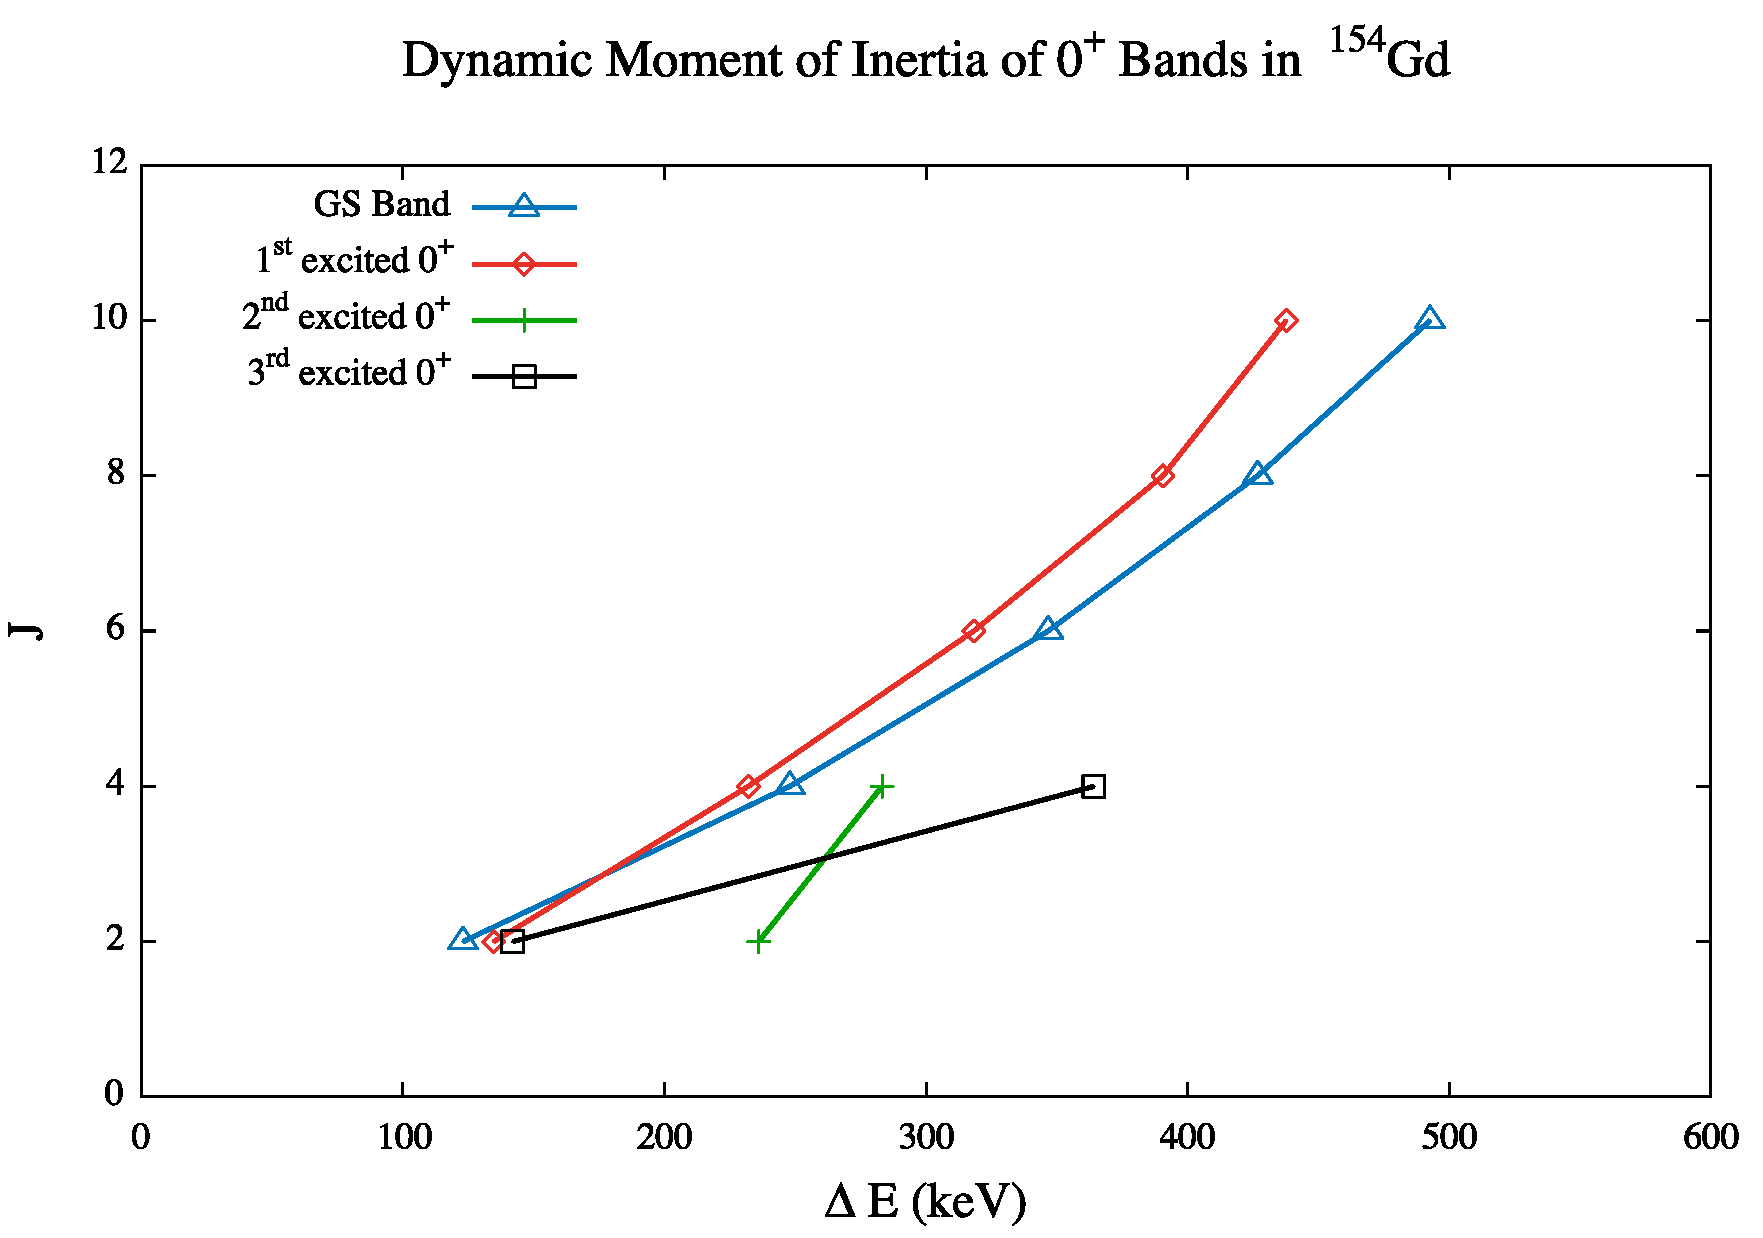
\includegraphics[scale=0.45]{154GdTablesAndFigs/154_Dynamic0.pdf}
    \caption{The dynamic moments of inertia of the four $0^+$ bands seen in the experiment. As is seen visually and with the slopes, the ground state band and the first excited $0^+$ band have very similar moments of inertia.}
    \label{fig:154_Dynamic0}
\end{figure}

\begin{figure}[!]
    \centering
    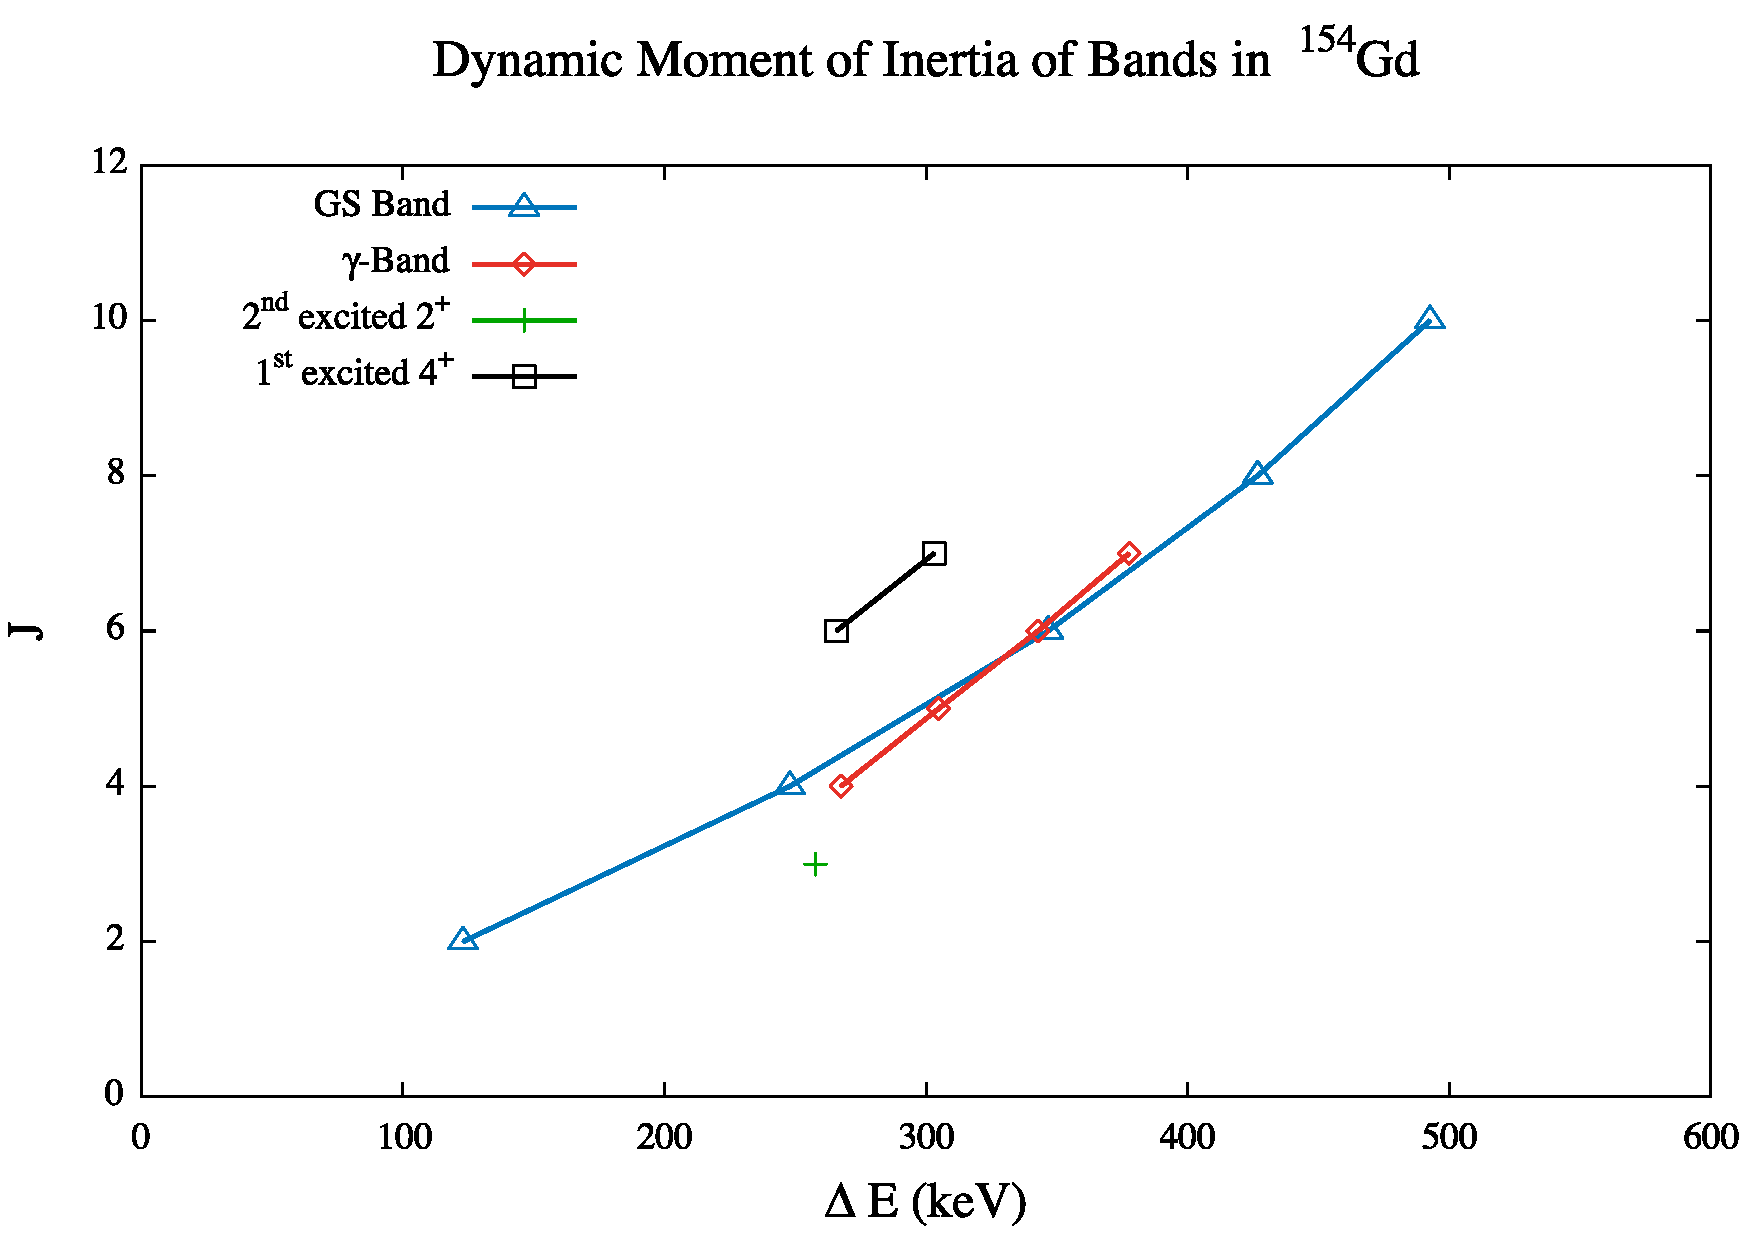
\includegraphics[scale=0.45]{154GdTablesAndFigs/154_Dynamic.pdf}
    \caption{The dynamic moments of inertia of the non-$0^+$ bands seen in the experiment. As is seen visually and with the slopes, the ground state band and the $\gamma$ band have similar moments of inertia. However, they do not overlap within their standard deviations.}
    \label{fig:154_Dynamic}
\end{figure}

\begin{table}[!]
    \centering
    \caption{Dynamic Moments of Inertia of Bands seen in $^{154}$Gd}
    \begin{tabular}{c|c}
        \toprule
        Band & Moment of Inertia  \\
        \hline
        Ground State & 0.0214 (15) \\
        1st excited $0^+$ & 0.0258 (19) \\
        2nd excited $0^+$ & 0.0424 \\
        3rd excited $0^+$ & 0.0090 \\
        $\gamma$-band & 0.0271 (3) \\
        2nd excited $2^+$ & 0.0155 \\
        1st excited $4^+$ & 0.0267 \\
        \bottomrule
    \end{tabular}
    \footnotesize
    \item Table \ref{tab:154_Dynamic}: List of the moments of inertia of the bands seen in $^{154}$Gd in this experiment. The moment of intertia is the slope in a least-squares linear regression. Those without error only had one or two points of energy difference, so the standard deviation of the slope could not be calculated. The ground state band the the first excited $0^+$ band agree within two standard deviations.
    \label{tab:154_Dynamic}
\end{table}

Figure \ref{fig:154_Dynamic0} shows the $0^+$ bands. The first excited $0^+$ band has a very similar slope to the ground state band, as seen both in Figure \ref{fig:154_Dynamic0} and Table \ref{tab:154_Dynamic}. The two bands agree within $2\sigma$. While the $\gamma$-band also appears similar in slope to the ground state band in Figure \ref{fig:154_Dynamic}, they do not overlap within $3\sigma$. The first $4^+$ excited band does have a slope within $2\sigma$ of the $\gamma$-band.

\subsection{Bands in $^{154}$Gd}
\label{sec:156_Dynamic}

To examine the structure of the band seen in this experiment, the dynamic moments of inertia can be compared. This is usually done at higher spins, but examination at lower spins can allow for more bands to be compared. The energy difference tracks linearly, with the slope being directly correlated to the moment of inertia of the band, as seen in Figures \ref{fig:156_Dynamic0} and \ref{fig:156_Dynamic}. The slopes of these bands are summarized in Table \ref{tab:156_Dynamic}. Slopes with an error had enough points to calculate the error on the slope. Those without error had only two points or, in the case of the second excited $2^+$ band, one point and the origin. These points each require two levels of the band to be known for calculation. The intercept was left to float, but not included, as it was in agreement with 0 in all cases where error could be calculated.

\begin{figure}[!]
    \centering
    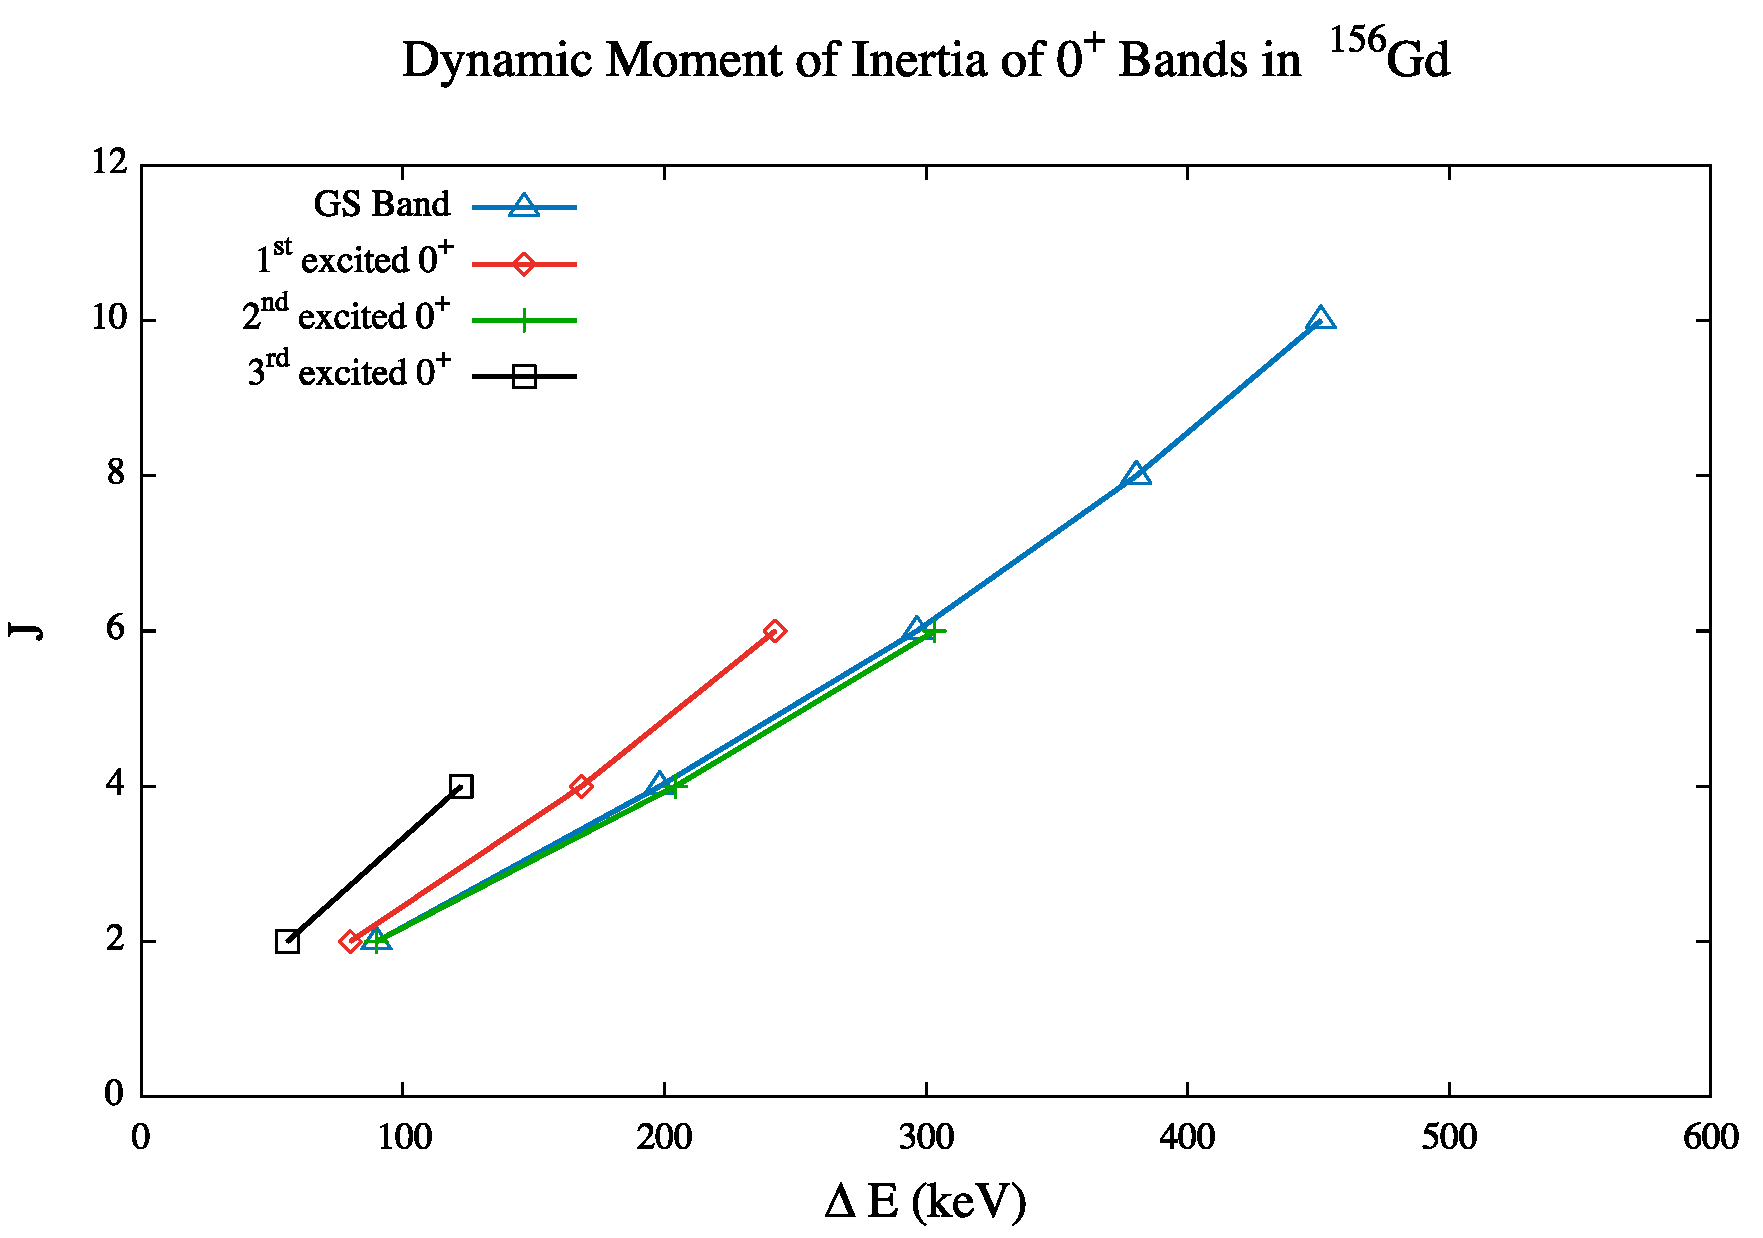
\includegraphics[scale=0.45]{156GdTablesAndFigs/156_Dynamic0.pdf}
    \caption{The dynamic moments of inertia of the four $0^+$ bands seen in the experiment. As is seen visually and with the slopes, the ground state band and the first excited $0^+$ band have very similar moments of inertia.}
    \label{fig:156_Dynamic0}
\end{figure}

\begin{figure}[!]
    \centering
    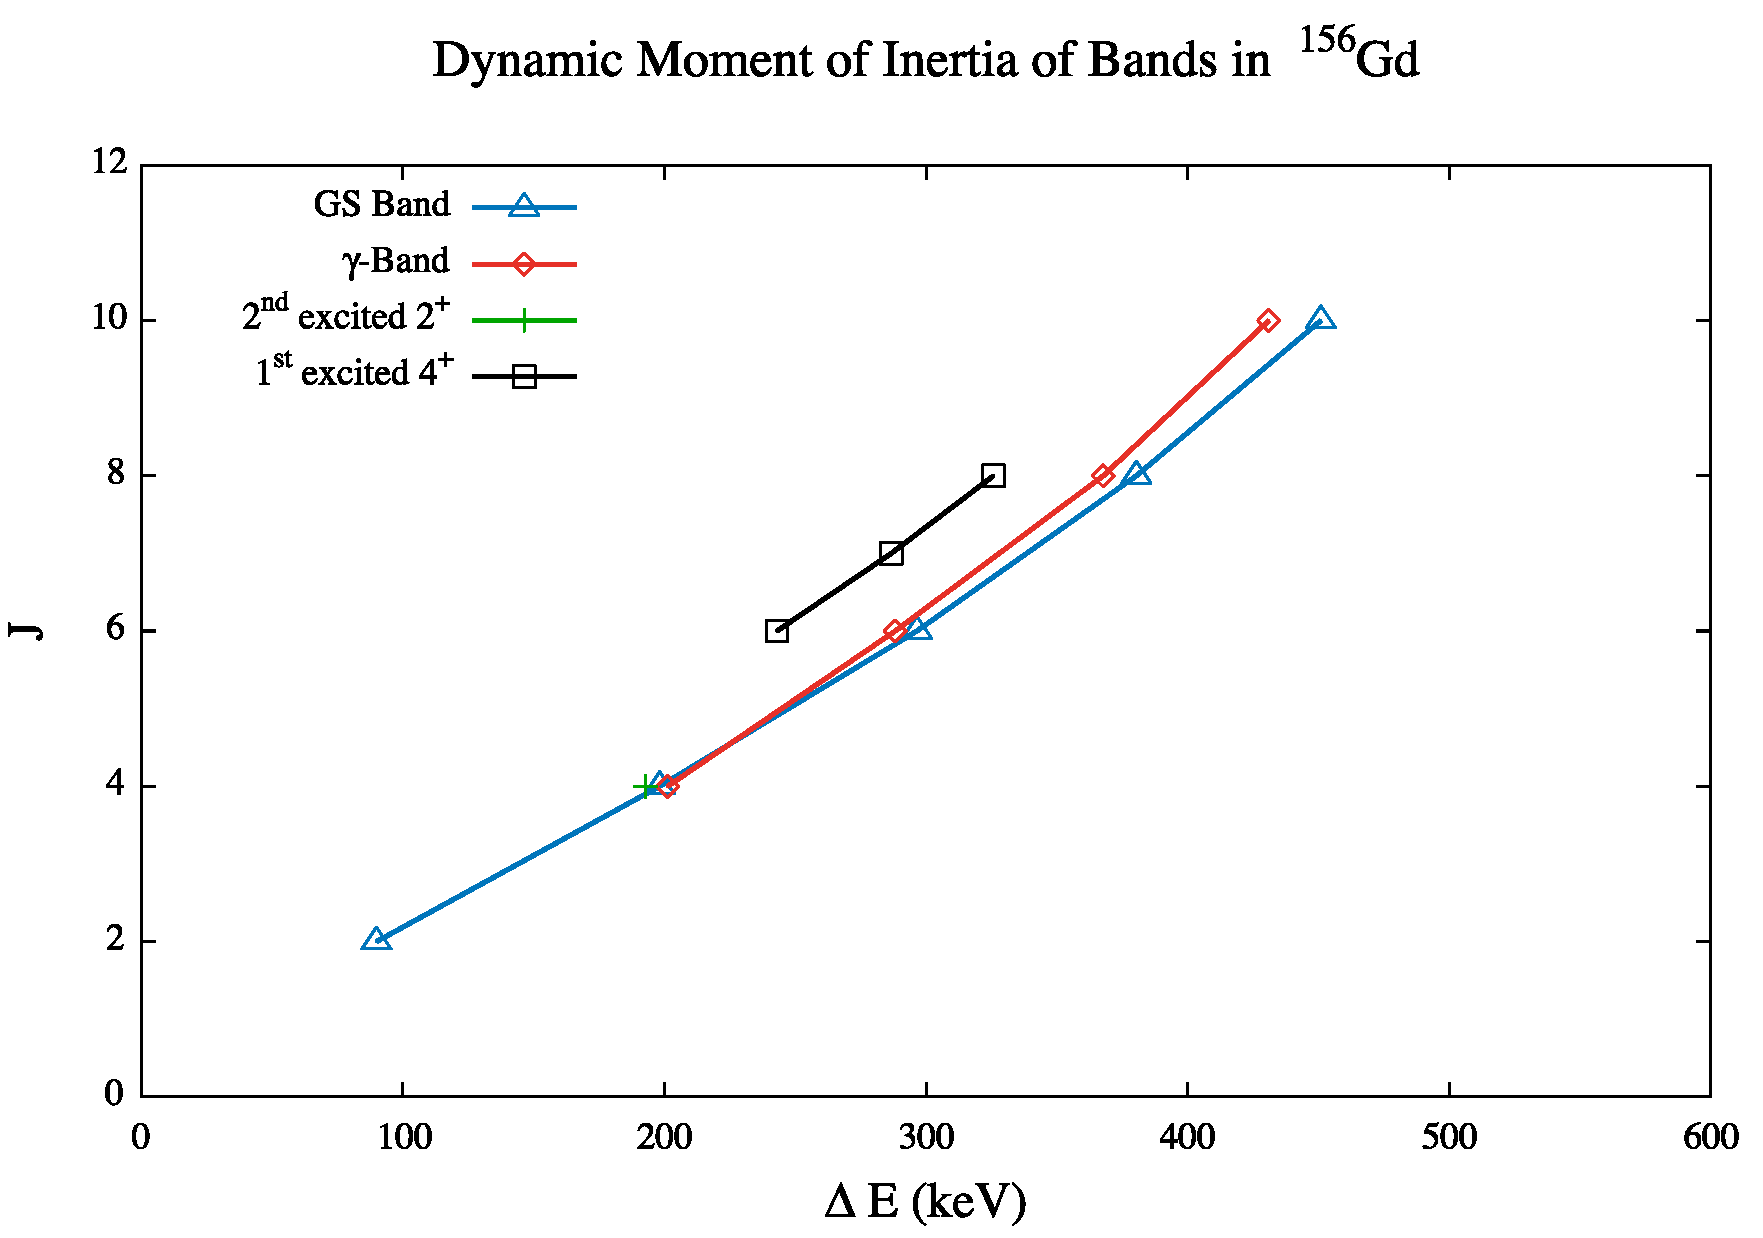
\includegraphics[scale=0.45]{156GdTablesAndFigs/156_Dynamic.pdf}
    \caption{The dynamic moments of inertia of the non-$0^+$ bands seen in the experiment. As is seen visually and with the slopes, the ground state band and the $\gamma$ band have similar moments of inertia, and overlap within two standard deviations.}
    \label{fig:156_Dynamic}
\end{figure}

\begin{table}[!]
    \centering
    \caption{Dynamic Moments of Inertia of Bands seen in $^{156}$Gd}
    \begin{tabular}{c|c}
        \toprule
        Band & Moment of Inertia  \\
        \hline
        Ground State & 0.0220 (11) \\
        1st excited $0^+$ & 0.0245 (13) \\
        2nd excited $0^+$ & 0.0187 (8) \\
        3rd excited $0^+$ & 0.0301 \\
        $\gamma$-band & 0.0259 (13) \\
        2nd excited $2^+$ & 0.0208 \\
        1st excited $4^+$ & 0.0242 (10)  \\
        \bottomrule
    \end{tabular}
    \footnotesize
    \item Table \ref{tab:156_Dynamic}: List of the moments of inertia of the bands seen in $^{156}$Gd in this experiment. The moment of inertia is the slope in a least-squares linear regression. Those without error only had one or two points of energy difference, so the standard deviation of the slope could not be calculated. The ground state band and the first excited $0^+$ band agree within two standard deviations. The same is true of the ground state band and both the $\gamma$-band and first excited $4^+$ band.
    \label{tab:156_Dynamic}
\end{table}

Figure \ref{fig:156_Dynamic0} shows the moments of inertia of the $0^+$ bands, including the ground state band. The first excited $0^+$ band has a very similar slope to the ground state band, as seen both in Figure \ref{fig:156_Dynamic0} and Table \ref{tab:156_Dynamic}. The two bands agree within $2\sigma$. The $\gamma$-band and the excited $4^+$ band also appear similar in slope to the ground state band in Figure \ref{fig:156_Dynamic}, and overlap within $2\sigma$. The first $4^+$ excited band is almost identical in slope to the first excited $0^+$ band. Both of these bands are about $1\sigma$ apart.